
\section{Review of Contraction Theory}

For your smooth start, we recommend you to begin with \cite{LOHMILLER:1998aa}.
The overview of contraction theory is presented in a review paper \cite{Tsukamoto:2021aa}.

\subsection{Basic Results of Contraction Theory for Deterministic Systems}

First, we start with the following deterministic systems:
\begin{equation}
    \ddtt{\bdx}
    = 
    \bdf(\bdx,t)
    ,
    \label{eq:sys}
\end{equation}
where $\bdf(\bdx,t)$ is an $n\times1$ sufficiently smooth non-linear vector function and $\bdx\in\R^n$ is the state vector.
The smooth property of $\bdf(\bdx,t)$ is essential to ensure the existence and uniqueness of the solution to \eqref{eq:sys} \cite[see, pp. 88-89]{Khalil:2002aa}.

\begin{figure}[!t]
    \centering
    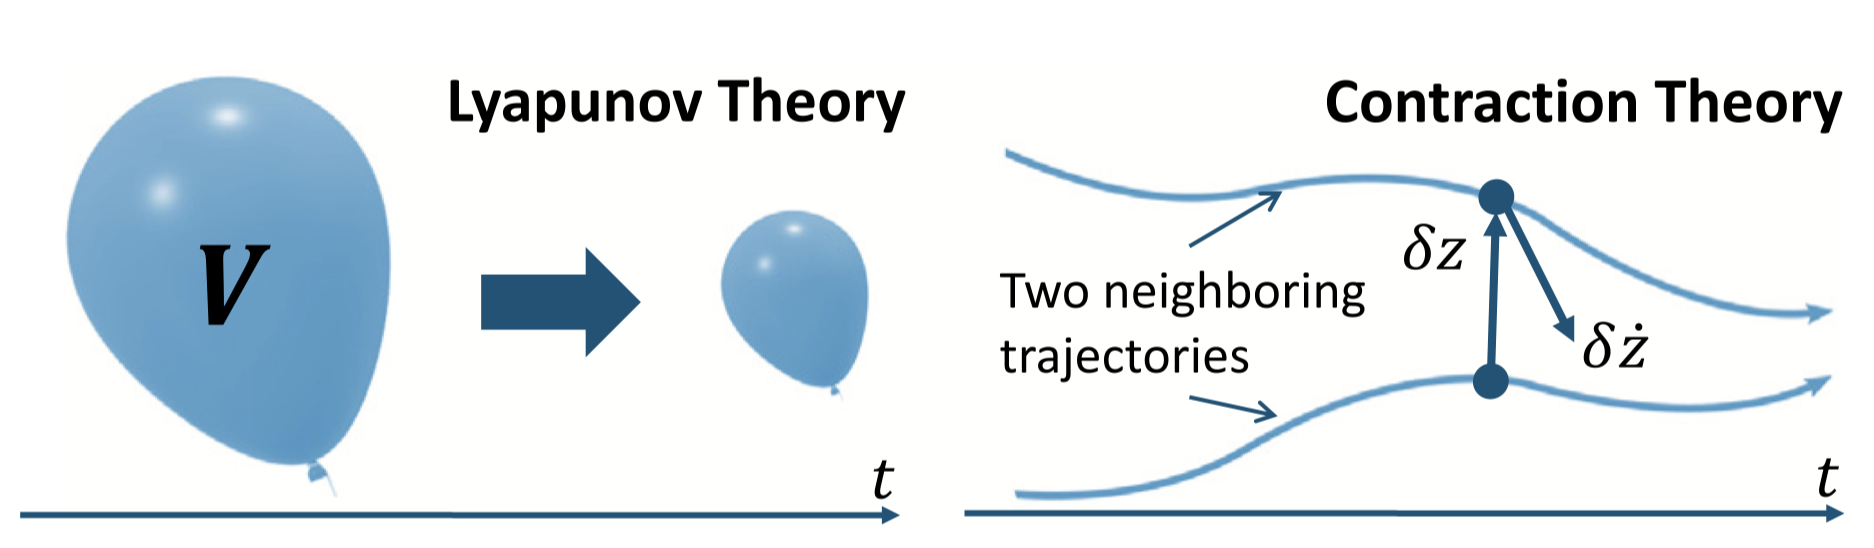
\includegraphics[width=0.5\textwidth]{figs/lyaVSctrac.png}
    \caption{
        Difference between Lyapunov and contraction theory \cite[Fig. 1]{Tsukamoto:2021aa}.
        The Lyapunov theory investigates the convergence to a single point and the contraction theory does regarding a single trajectory.
    }
    \label{fig:lyaVSctrac}
\end{figure}

The biggest difference between the traditional Lyapunov theory and the contraction theory is that the contraction theory investigates the convergence of the state trajectory to a single trajectory (contraction behavior), while the Lyapunov theory focuses on the convergence of the state trajectory to a single point \ie see, Fig.~\ref{fig:lyaVSctrac}.
For this, motivated by the calculus of variations \cite[Chap. 4]{Kirk:2004aa}, \eqref{eq:sys} can be rewritten as differential dynamics using \textit{differential displacement} $\delta\bdx$ as follows:
\begin{equation}
    \ddtt\delta\bdx
    =
    \tpfpx(\bdx,t)
    \delta\bdx
    .
    \label{eq:diff_sys}
\end{equation}
For your information, $\delta\bdx$ is an infinitesimal displacement at \textit{fixed time}.

\subsubsection{Notable Definitions}

Before we present the fundamental theorem of contraction theory, we introduce the following definitions.
One can re-visit this section while reading further.

\begin{definition}[see, Def. 2.2 \cite{Tsukamoto:2021aa}]  
    If any two trajectories $\mv\xi_1(t)$ and $\mv\xi_2(t)$ of \eqref{eq:sys} converge to a single trajectory, then the system \eqref{eq:sys} is said to be \textit{incrementally exponentially stable}, if $\exists C,\alpha>0$, subject to the following holds:
    \begin{equation}      
        \norm{\mv\xi_1(t)-\mv\xi_2(t)}
        \le 
        C
        \norm{\mv\xi_1(0)-\mv\xi_2(0)}
        \exp^{-\alpha t}
        ,\ \forall t\in\R_{\ge 0}
        .
    \end{equation}
    The result of Theorem \ref{thm:ctrac:main} equivalently implies the incremental exponential stability, since we have $\norm{\mv\xi_1(t)-\mv\xi_2(t)}= \norm{\int_{\mv\xi_1(t)}^{\mv\xi_2(t)}\delta\bdx(t)}$.
    \label{def:inc_exp_stable}
\end{definition}

\begin{definition}
    Let $\mm\Theta(\bdx,t)$ be a smooth coordinate transformation of $\delta\bdx$ to $\delta\bdz$, \ie $\delta\bdz = \Theta(\bdx,t)\delta\bdx$.
    Then, a symmetric continuously differentiable matrix $\mm M(\bdx,t):=\mm\Theta(\bdx,t)^\top\mm\Theta(\bdx,t)$ is said to be a \textit{metric} of the system \eqref{eq:sys}.
    \label{def:metric}
\end{definition}

\begin{definition}
    The covariant derivative of $\mv f(\bdx,t)$ in $\delta\bdx$ coordinate is represented as 
    \begin{equation}
        \mm F
        :=
        \left(
            \ddtt\mm\Theta
            +
            \mm\Theta\tpfpx
        \right)
        \mm\Theta^{-1}
        ,
    \end{equation}
    and is called the \textit{generalized Jacobian}.
    This can be easily derived by differentiating $\delta\bdz = \Theta(\bdx,t)\delta\bdx$ with respect to $t$, leading to $\ddtt\bdz=\mm F\bdz$.
\end{definition}

\subsubsection{Fundamental Theorem of Contraction Theory}

The following theorem presents the fundamental theorem of contraction theory and corresponding necessary and sufficient condition for exponential convergence of the differential system \eqref{eq:diff_sys}.

\begin{theorem}[see, T. 2.1 \cite{Tsukamoto:2021aa}]
    If $
        \exists \mm{M}(\bdx,t)
        =
        \mm\Theta(\bdx,t)^\top
        \mm\Theta(\bdx,t)
        > 0, \forall \bdx,t
    $ where $\mm\Theta(\bdx,t)$ defines a smooth coordinate transformation of $\delta\bdx$ to $\delta\bdz$, \ie $\delta\bdz = \Theta(\bdx,t)\delta\bdx$, subject to the following equivalent conditions holds for $\exists\alpha\in\R_{>0},\ \forall \bdx,t$:
    \begin{subequations}
        \begin{align}
            \lambda_{\max} (
                \mm F(\bdx,t)
            )
            =
            \lambda_{\max} 
            \left(
                \left(    
                \ddtt \mm\Theta
                +
                \mm\Theta\tpfpx
                \right)
                \mm\Theta^{-1}
            \right)
            \le&
            -\alpha
            ,
        \label{eq:ctrac:metric:F}
            \\
            \ddtt \mm M
            +
            \mysym(\mm M\tpfpx)
            \le&
            -2\alpha\mm M
            ,
        \label{eq:ctrac:metric:M}
        \end{align}
        \label{eq:ctrac:metric}
    \end{subequations}
    where the arguments of $\mm M(\bdx,t)$ and $\mm F(\bdx,t)$ are omitted for simplicity, then, the system \eqref{eq:sys} is said to be contracting with an exponential rate $\alpha$, \ie all trajectories of \eqref{eq:sys} converge to a single trajectory.
    The converse is also true.
    \label{thm:ctrac:main}
\end{theorem}

\begin{proof}
    Taking time derivative of a differential Lyapunov function of $\delta\bdx$, $V=\delta\bdz^\top\bdz=\delta\bdx^\top\mm M\delta\bdx$, using the differential dynamics \eqref{eq:diff_sys}, we have
    \begin{equation}
        \begin{aligned}
            \ddtt V (\bdx, \delta\bdx, t)
            =&
            \delta\bdx^\top
            \left(
                \ddtt\mm M
                +
                \mysym(\mm M\tpfpx)
            \right)
            \delta\bdx
            =
            2
            \delta\bdz^\top
            \mm F
            \delta \bdz
            \\
            \le&
            -2\alpha
            \delta\bdx^\top
            \mm M
            \delta\bdx
            =
            -
            2\alpha
            \delta\bdz^\top
            \delta\bdz
            =
            -2\alpha V
            .
        \end{aligned}
    \end{equation}
    According to the comparison lemma (Lemma \ref{lem:comparison}), we have $V(t)\le V(0)e^{-2\alpha t}$, which then yields $\norm{\delta\bdz(t)}^2\le\norm{\delta\bdz(0)}^2e^{-2\alpha t}$ and $\norm{\delta\bdz(t)}\le\norm{\delta\bdz(0)}e^{-\alpha t}$.
    This implies that any infinitesimal displacement $\delta\bdz$ and $\delta\bdx$ converges to zero exponentially with rate $\alpha$.
    Note that the initial conditions are exponentially "forgotten" as time goes on.
    The proof of the converse can be found in \cite[Sec. 3.5]{LOHMILLER:1998aa}.
\end{proof}

It is notable that the unboundedness of the metric $\mm M(\bdx, t)$ does not create any problem in a technical sense.
This is because, the dynamics of $\mm M(\bdx, t)$ is linear with infinite escape time.
Therefore, it can be handled by renormalizing the metric $\mm M(\bdx, t)$.

\hfill

Theorem \ref{thm:ctrac:main} can also be proven by using the transformed squared length integrated over two arbitrary solutions of \eqref{eq:sys}.
The following theorem presents the alternative proof of Theorem \ref{thm:ctrac:main}.

\begin{theorem}[see, T. 2.3 \cite{Tsukamoto:2021aa}]
    Let $\mv{\xi}_1(t)$ and $\mv{\xi}_2(t)$ be two solutions of \eqref{eq:sys}, and define the transformed squared length with $\mm M(\bdx,t)$ of Theorem \ref{thm:ctrac:main} as follows:
    \begin{equation}
        V_{sl}(\bdx,\delta\bdx,t)
        =
        \textstyle\int_{\mv{\xi}_1(t)}^{\mv{\xi}_2(t)}
        \norm{\delta\bdz}^2
        =
        \textstyle\int_0^1
        \pptfrac{\bdx}{\mu}^\top
        \mm M(\bdx,t)
        \pptfrac{\bdx}{\mu}
        \der\mu
        ,
        \label{eq:Vsl}
    \end{equation}
    where $\bdx$ is a smooth path parameterized as $\bdx(\mu=0,t)=\mv\xi_1(t)$ and $\bdx(\mu=1,t)=\mv\xi_2(t)$ by $\mu\in\{0,1\}$.
    Also, define the path integral with the transformation $\mm\Theta(\bdx,t)$ for $\mm M(\bdx,t)=\mm\Theta(\bdx,t)^\top\mm\Theta(\bdx,t)$ as follows:
    \begin{equation}
        V_{l}(\bdx,\delta\bdx,t)
        =
        \textstyle\int_{\mv{\xi}_1(t)}^{\mv{\xi}_2(t)}
        \norm{\delta\bdz}
        =
        \textstyle\int_{\mv{\xi}_1(t)}^{\mv{\xi}_2(t)}
        \norm{\mm\Theta(\bdx,t)\delta\bdx}
        .
        \label{eq:Vl}
    \end{equation}
    Then, \eqref{eq:Vsl} and \eqref{eq:Vl} satisfy the following inequality:
    \begin{equation}
        \norm{\mv\xi_1(t)-\mv\xi_2(t)}
        =
        \norm{
            \textstyle\int_{\mv{\xi}_1(t)}^{\mv{\xi}_2(t)}
            \delta\bdx
        }
        \le
        \tfrac{V_{l}}{\sqrt{\underbar{m}}}
        \le
        \sqrt{\tfrac{V_{sl}}{\underbar{m}}}
        ,
    \end{equation}
    where $\mm M(\bdx,t) \ge \underbar{m}\mm I_n,\ \forall \bdx, t$ for $\exists\underbar{m}\in\R_{>0}$ and Theorem \ref{thm:ctrac:main} can also be proven by using \eqref{eq:Vsl} and \eqref{eq:Vl} as a Lyapunov-like function, resulting in incremental exponential stability of the system \eqref{eq:sys} (see, Definition \ref{def:inc_exp_stable}).
    Note that the shortest path integral $V_l$ of \eqref{eq:Vl} with a parameterized state $\bdx$ (\ie $\inf{V_l}=\sqrt{\inf{V_{sl}}}$) defines the Riemannian distance and the path integral of a minimizing geodesic.
\end{theorem}

\begin{proof}
    ...
\end{proof}

\hfill

\begin{example}
    Consider the following system:
    \begin{equation}
        \ddt
        \begin{bmatrix}
            x_1\\
            x_2
        \end{bmatrix}
        =
        \begin{bmatrix}
            -1 & x_1\\
            -x_1 & -1
        \end{bmatrix}
        \begin{bmatrix}
            x_1\\
            x_2
        \end{bmatrix}
        .
    \end{equation}
\end{example}

\hfill

However, aforementioned theorems are limited to the convergence of the state trajectory to a single trajectory.
In the next section, we introduce the partial contraction theory to investigate the convergence of the state trajectory to a desired trajectory.

\subsubsection{Partial Contraction}

\cite{Wang:2004aa,Jouffroy:2004aa}

\subsection{Basic Results of Contraction Theory for Stochastic Systems}
